\documentclass{article}
\usepackage[utf8]{inputenc}
\usepackage{amsmath,amssymb}
\usepackage{cancel}
\usepackage{makecell}
\usepackage[a4paper, total={6in, 9in}]{geometry}
\usepackage{authblk}
\usepackage{graphicx}
\graphicspath{{.}}
\author{Zihan Zhao}
\affil{1001103708}
\title{Homework 4}
\date{}
\begin{document}
\maketitle
\renewcommand{\thesubsection}{(\alph{subsection})}
\section{Multilayer Perceptron}
There are 2 units on input layer, 6 units on hidden layer and 2 units on output layer. The $W,b$ for each layer edges are as following:
\begin{align*}
    W^{(1)} &= 
    \begin{bmatrix}
        1 & -1\\
        -1 & 1\\
        1 & 0\\
        0 & 1\\
        -1 & 0\\
        0 & -1\\
    \end{bmatrix}
    b^{(1)} = 
    \begin{bmatrix}
        0\\
        0\\
        0\\
        0\\
        0\\
        0\\
    \end{bmatrix}\\
    W^{(2)} &= 
    \begin{bmatrix}
        -\frac{1}{2} & -\frac{1}{2} & \frac{1}{2} & \frac{1}{2} & -\frac{1}{2} & -\frac{1}{2}\\
        \frac{1}{2} & \frac{1}{2} & \frac{1}{2} & \frac{1}{2} & -\frac{1}{2} & -\frac{1}{2}\\
    \end{bmatrix}
    b^{(2)} = 
    \begin{bmatrix}
        0\\
        0\\
    \end{bmatrix}\\
\end{align*}
How does it work?\\
\begin{align*}
h1&=ReLU(x_1-x_2)\\
h2&=ReLU(x_2-x_1)\\
h3&=ReLU(x_1)\\
h4&=ReLU(x_2)\\
h5&=ReLU(-x_1)\\
h6&=ReLU(-x_2)\\
\intertext{We can get $y_1$, $y_2$}
y1&=-\frac{1}{2}h1 + -\frac{1}{2}h2 + \frac{1}{2}h3 + \frac{1}{2}h4 + -\frac{1}{2}h5 + -\frac{1}{2}h6\\
&=-\frac{1}{2}h1 + -\frac{1}{2}h2 + \frac{1}{2}(h3-h5) + \frac{1}{2}(h4-h6)\\
&=-\frac{1}{2}h1 + -\frac{1}{2}h2 + \frac{1}{2}(max(0,x_1)-max(0,-x_1)) + \frac{1}{2}(max(0,x_2)-max(0,-x_2))\\
\intertext{If $x_1 \geq 0$, $max(0,x_1)-max(0,-x_1)=x_1-0=x_1$;}
\intertext{If $x_1 < 0$, $max(0,x_1)-max(0,-x_1)=0-(-x_1)=x_1$; So is $x_2$. Then,}\\
y1&=-\frac{1}{2}h1 + -\frac{1}{2}h2 + \frac{1}{2}x_1+\frac{1}{2}x_2\\
y2&=\frac{1}{2}h1 + \frac{1}{2}h2 + + \frac{1}{2}x_1+\frac{1}{2}x_2\\
\intertext{If $x_1 \geq x_2$,}
h1&=x_1-x_2\\
h2&=0\\
\intertext{Then,}
y1&=-\frac{1}{2}(x_1-x_2) + -\frac{1}{2}*0 + \frac{1}{2}x_1+\frac{1}{2}x_2\\
&=-\frac{1}{2}x_1+ -\frac{1}{2}(-x_2) + \frac{1}{2}x_1+\frac{1}{2}x_2\\
&=x_2\\
y2&=\frac{1}{2}(x_1-x_2) + \frac{1}{2}*0 + \frac{1}{2}x_1+\frac{1}{2}x_2\\
&=x_1\\
\intertext{If $x_1 < x_2$,}
h1&=0\\
h2&=x_2-x_1\\
\intertext{Then,}
y1&=-\frac{1}{2}(x_2-x_1) + \frac{1}{2}x_1+\frac{1}{2}x_2\\
&=x_1\\
y2&=\frac{1}{2}(x_2-x_1) + \frac{1}{2}x_1+\frac{1}{2}x_2\\
&=x_2\\
\intertext{They are sorted in order.}
\end{align*}
\section{Backprop}
\subsection{}
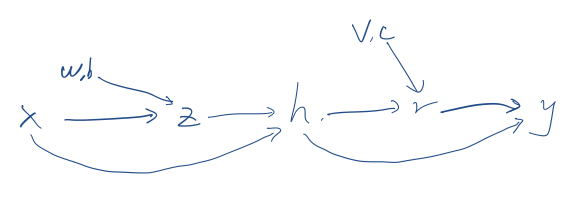
\includegraphics[width=\textwidth,height=\textheight,keepaspectratio]{cg.png}
\subsection{}
Assume we know $\overline{y} = \frac{\mathrm{d} L}{\mathrm{d} y} $
\end{document}
